% aha-2017-slcs-slides.Rnw

%---------------------------------------------------------------
% Preamble
% --------------------------------------------------------------
%
% NOTE: See rice-sample.tex written by Daina Chiba at Rice University for formatting and preamble code that I copied, http://ricebeamer.dynaman.net/
\documentclass[pdf]{beamer}\usepackage[]{graphicx}\usepackage[]{color}
%% maxwidth is the original width if it is less than linewidth
%% otherwise use linewidth (to make sure the graphics do not exceed the margin)
\makeatletter
\def\maxwidth{ %
  \ifdim\Gin@nat@width>\linewidth
    \linewidth
  \else
    \Gin@nat@width
  \fi
}
\makeatother

\definecolor{fgcolor}{rgb}{0.345, 0.345, 0.345}
\newcommand{\hlnum}[1]{\textcolor[rgb]{0.686,0.059,0.569}{#1}}%
\newcommand{\hlstr}[1]{\textcolor[rgb]{0.192,0.494,0.8}{#1}}%
\newcommand{\hlcom}[1]{\textcolor[rgb]{0.678,0.584,0.686}{\textit{#1}}}%
\newcommand{\hlopt}[1]{\textcolor[rgb]{0,0,0}{#1}}%
\newcommand{\hlstd}[1]{\textcolor[rgb]{0.345,0.345,0.345}{#1}}%
\newcommand{\hlkwa}[1]{\textcolor[rgb]{0.161,0.373,0.58}{\textbf{#1}}}%
\newcommand{\hlkwb}[1]{\textcolor[rgb]{0.69,0.353,0.396}{#1}}%
\newcommand{\hlkwc}[1]{\textcolor[rgb]{0.333,0.667,0.333}{#1}}%
\newcommand{\hlkwd}[1]{\textcolor[rgb]{0.737,0.353,0.396}{\textbf{#1}}}%
\let\hlipl\hlkwb

\usepackage{framed}
\makeatletter
\newenvironment{kframe}{%
 \def\at@end@of@kframe{}%
 \ifinner\ifhmode%
  \def\at@end@of@kframe{\end{minipage}}%
  \begin{minipage}{\columnwidth}%
 \fi\fi%
 \def\FrameCommand##1{\hskip\@totalleftmargin \hskip-\fboxsep
 \colorbox{shadecolor}{##1}\hskip-\fboxsep
     % There is no \\@totalrightmargin, so:
     \hskip-\linewidth \hskip-\@totalleftmargin \hskip\columnwidth}%
 \MakeFramed {\advance\hsize-\width
   \@totalleftmargin\z@ \linewidth\hsize
   \@setminipage}}%
 {\par\unskip\endMakeFramed%
 \at@end@of@kframe}
\makeatother

\definecolor{shadecolor}{rgb}{.97, .97, .97}
\definecolor{messagecolor}{rgb}{0, 0, 0}
\definecolor{warningcolor}{rgb}{1, 0, 1}
\definecolor{errorcolor}{rgb}{1, 0, 0}
\newenvironment{knitrout}{}{} % an empty environment to be redefined in TeX

\usepackage{alltt}

\usetheme{Frankfurt}
\usecolortheme{beetle}
\setbeamersize{text margin left=10pt,text margin right=10pt} %set margin sizes


\usepackage[english]{babel}
\usepackage[latin1]{inputenc}
\usepackage{bm}
\usepackage{blindtext}
\usepackage{scrextend}
\addtokomafont{labelinglabel}{\sffamily}
\usepackage{csquotes}
\usepackage{booktabs}

\usepackage{graphicx}% http://ctan.org/pkg/graphicx

\setbeamercolor{bibliography entry title}{fg=black,bg=black}% see http://tex.stackexchange.com/questions/71352/beamer-undefined-color-local-structure
\setbeamercolor{bibliography entry location}{fg=white}
\setbeamercolor{bibliography entry note}{fg=white}
\setbeamertemplate{caption}[numbered]

% got from http://tex.stackexchange.com/questions/48023/mimic-bibtex-apalike-with-biblatex-biblatex-apa-broken
\PassOptionsToPackage{
        style=numeric,
        hyperref=true,
        backend=bibtex,
        maxbibnames=1,
        firstinits=true,
        uniquename=init,
        maxcitenames=2,
        parentracker=true,
        url=false,
        doi=true,
        isbn=false,
        eprint=false,
        backref=false,
        pagetracker=true,
        citetracker=true
            }{biblatex}
% see the following link for info on biblatex sort order issue: 
% http://tex.stackexchange.com/questions/51434/biblatex-citation-order
\usepackage[natbib=true, sorting=none]{biblatex}
\addbibresource{lit}
\renewcommand*{\bibfont}{\scriptsize}


% see http://tex.stackexchange.com/questions/43083/author-year-abbr-journal-name-as-citation-style
\DeclareCiteCommand{\longcite}{(}{%
    \printnames[author]{author}, \printfield{year})}{}{}%

\newcommand{\customcite}[1]{\citeauthor{#1}, \citetitle{#1}, \citeyear{#1}}
\newcommand{\customcitetwo}[1]{\citeauthor{#1}, \citeyear{#1}}

\renewcommand{\footnotesize}{\tiny}  % change font size of citation
\renewcommand\multicitedelim{\addsemicolon\space} % This doesn't seem to work, but see http://tex.stackexchange.com/questions/167665/multiple-references-with-footfullcite



%\usepackage{fontspec} % have to compile with XeLaTeX
%\setmainfont{Arial}
\usepackage[T1]{fontenc}
\usepackage{helvet}
\renewcommand{\familydefault}{\sfdefault} % get something like Arial

\usepackage{amsmath,amsthm, amssymb, latexsym}
\usepackage{wrapfig}

\usepackage{array,booktabs,tabularx}
\newcolumntype{Z}{>{\centering\arraybackslash}X} % centered tabularx columns

\usepackage[shortlabels]{enumitem}

% \setlist[description]{style=nextline}
\setlist[itemize]{label=$\bullet$}

\usepackage[framemethod=TikZ]{mdframed}
\mdfdefinestyle{MyFrame}{%
    linecolor=carolinablue,
    outerlinewidth=4pt,
    roundcorner=20pt,
    innerrightmargin=20pt,
    innerleftmargin=20pt,
    backgroundcolor=carolinablue!20}
    
% comment 
\newcommand{\comment}[1]{}

% (relative) path to the figures
%\graphicspath{{figs/}}




% This is based on the template at http://www-i6.informatik.rwth-aachen.de/~dreuw/latexbeamerposter.php

% --------------------------------------------------------------------------------------% 
% Title, author, date, etc.
% --------------------------------------------------------------------------------------% 
% see http://tex.stackexchange.com/questions/9740/how-can-i-add-vertical-space-to-a-beamercolorbox-to-make-it-align-with-another-o
\title{Lipid-related Genetic Variants and Lipid Outcomes in a Cohort of Chilean Children} 
\author[vonholle@unc.edu]{Ann Von Holle, Anne Justice, Misa Graff, Kari E. North, UNC, Chapel Hill, NC; Estela Blanco, Sheila Gahagan, UCSD, San Diego, CA; B\'arbara Angel, Unidad de Nutrici\'on P\'ublica INTA, Univ de Chile, Santiago, Chile; Jos\'e Luis Santos, Pontificia Univ Cat\'olica de Chile, Santiago, Chile}


% -------------------------------------------------------------------------------------%
% Contents
% -------------------------------------------------------------------------------------%
\IfFileExists{upquote.sty}{\usepackage{upquote}}{}
\begin{document}

\begin{frame}
\titlepage
\centering
\end{frame}

\section{Introduction}
\subsection{Introduction}

\begin{frame}{Lipid concentrations}
\large  
                \begin{itemize} 
                    \item Are a recognized heritable risk factor for cardiovascular disease (CVD)
                    \item Associate with >150 loci in adults
                    \item Vary across ancestral groups
                    \item Include high density lipoprotein cholesterol (HDL-C), low density lipoprotein cholesterol (LDL-C) and triglycerides (TG).
                    \end{itemize}
    
\end{frame}


\begin{frame}{Genetic architecture across racial/ethnic groups}

\begin{block}{Genetic Architecture}
'...Loci influencing the trait, direction and magnitude of genetic effects, and proportions of phenotypic variation explained...'.'$^1$
\end{block}

  \begin{itemize}
      \item Genetic architecture underlying lipid traits is similar across ancestral groups for adults.\footfullcite{coram_genome-wide_2013-1}
      \item Unclear if lipid-related loci associations found in adults extend to younger age groups.
      
      \begin{itemize}
        \item One European study establishes continuity of associations across the age spectrum\footfullcite{tikkanen_association_2011}, but evidence is sparse in Hispanic/Latino (HL) populations.
        \end{itemize}
      \end{itemize}
    
\end{frame}

% ------------------------------

\section{Aims}
\subsection{Aims}

\begin{frame}{Aims}
        \begin{description}
            \item[Aim 1] Estimate association between lipid risk variants first identified in adults and adolescent lipid traits from Santiago Longitudinal Cohort Study (SLCS), a Chilean infancy cohort\footfullcite{lozoff_behavioral_2003}.
            \item[Aim 2] Compare results between SLCS and Cardiovascular Risk in Young Finns Study Cohort\footfullcite{tikkanen_association_2011}.
            \end{description}

        \end{frame}

\subsection{Sample}
\begin{frame}{Sample}

\begin{columns}[T] % align columns
\begin{column}{.35\textwidth}
\centering
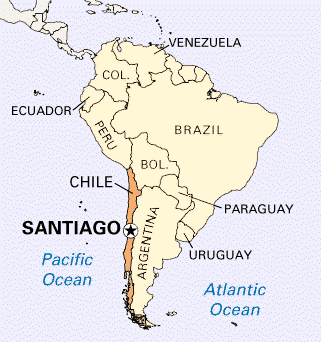
\includegraphics[scale=0.6]{santiago-map.png}
\end{column}%
\hfill%
\begin{column}{.6\textwidth}

\vspace{-1em}

 \begin{itemize}\small{
          \item 1,645 infants began SLCS between 1991-1996
          \item \raggedright Current sample recruited from n=888, which were 2 of 3 randomized control trial groups
          \item  n=677 with infancy and adolescent data and of those n=546 with genotyped data in analyses that follow
          \item Low to middle income status in Chile.
          \item Ancestrally mixed American Indian and Spanish descent families
          \item Lipid traits measured after overnight fasting at mean age 17 years.}
          \end{itemize}

\end{column}%
\end{columns}

\end{frame}
        

% ------------------------------
\section{Methods}

\subsection{Methods}

\begin{frame}{Methods}
        
        \begin{enumerate}[1.]
          \item Test additive association between lipid traits and adequately powered single risk variants.
            \begin{itemize}
              \item 76 common \textbf{lipid variants} selected from a European genome-wide meta-analysis with strongest independent signal\footfullcite{buscot_combined_2016}.
              \item Association tests include 6 \textbf{single variants} with \textit{a priori} power > 0.80.
            \end{itemize}
          \item Assess the association of weighted genetic risk scores (wGRS) on lipid traits using linear regression model.
       \begin{itemize}
           \item \textbf{Coefficients} for wGRS and power calculations based on European adult association studies\footfullcite{teslovich_biological_2010}.
              \end{itemize}

          \item Characterize proportion of variance explained by lipid variants.
          \end{enumerate}
\end{frame}

% >>>>>>>>>>>>>>>>>>>>>>>>>>>>>>>

\begin{frame}{1. Association tests}

\begin{itemize}
  \item We assessed single variant associations using linear regression for HDL-C, LDL-C, TG, assuming an additive genetic model, adjusted for sex and ancestry (via principal components).
\end{itemize}

\begin{description}
  \item[Sample Model for HDL] $$HDL_i = \beta_0 + SNP_i \beta_1 + sex_i \beta_2 + ANCESTRY_i \boldsymbol{\beta} + \epsilon_i$$
\end{description}

\begin{itemize}
  \item $SNP_i$ represents one single nucleotide polymorphism (SNP) with 'genotypes were coded as 0, 1, or 2 when directly genotyped or as a predicted allele dosage (range, 0-2) when imputed.' \footfullcite{tikkanen_association_2011}
    
  \item Only six variants from the Chilean sample met the \textit{a priori} threshold of power > 0.8 to detect an association based on effect sizes from GWAS \footfullcite{teslovich_biological_2010}.
  \end{itemize}

\end{frame}

% >>>>>>>>>>>>>>>>>>>>>>>>>>>>>>>

\begin{frame}{2. Polygenic risk scores}

\begin{itemize}
  \item Regress phenotypes onto weighted trait-specific genetic risk scores (GRS).
  \end{itemize}

\begin{description}
  \item[Sample model for HDL:] $HDL_i = \beta_0 + \beta_1 GRS1_i + \epsilon_i$
  \item[GRS for HDL-C:] \scriptsize ($0.48 * rs4660293 + 0.49 * rs2814944 + 0.59 * rs4731702 + 0.41 * rs2923084 + 0.4 * rs7134375 + 0.44 * rs7134594 + 1.45 * rs1532085 + 3.39 * rs3764261 + 0.45 * rs2925979 + 0.42 * rs4148008 + 0.39 * rs4129767 + 0.64 * rs737337 + 1.88 * rs1800961 + 0.93 * rs6065906 + 0.47 * rs1689800 + 0.61 * rs4846914 + 0.68 * rs12328675 + 0.46 * rs2972146 + 0.49 * rs6450176 + 0.39 * rs605066 + 1.95 * rs1084651 + 1.21 * rs9987289 + 0.44 * rs2293889 + 0.65 * rs581080 + 0.94 * rs1883025 + 0.78 * rs3136441 + 0.86 * rs4759375 + 0.44 * rs4765127 + 0.61 * rs838880 + 0.39 * rs2652834 + 1.27 * rs16942887 + 0.48 * rs11869286 + 1.31 * rs7241918 + 0.42 * rs12967135 + 0.45 * rs7255436 + 0.83 * rs386000 + 0.46 * rs181362 + 0.84 * rs13107325) / 29.79$
\end{description}

\begin{itemize}
  \item All GRS are standardized in the regression models: regression coefficient for GRS indicates a one unit change in SD of GRS.
  \end{itemize}
  
\end{frame}
  
% >>>>>>>>>>>>>>>>>>>>>>>>>>>>>>>

\begin{frame}{3. Proportion of variance explained by SNPs}

\begin{itemize}
  \item Linear models containing all lipid-related SNPs related to a specific phenotype, such as HDL-C, will be covariates. 
  \item The continuous lipid phenotype is the outcome. 
  \item Differences in R$^2$ will be calculated between models with and without the SNPs to estimate h$^2$.
\end{itemize}

\begin{description}
  \item[Model for HDL:] \scriptsize$HDL_i$ = b0 + b1 * rs4660293 + b2 * rs2814944 + b3 * rs4731702 + b4 * rs2923084 + b5 * rs7134375 + b6 * rs7134594 + b7 * rs1532085 + b8 * rs3764261 + b9 * rs2925979 + b10 * rs4148008 + b11 * rs4129767 + b12 * rs737337 + b13 * rs1800961 + b14 * rs6065906 + b15 * rs1689800 + b16 * rs4846914 + b17 * rs12328675 + b18 * rs2972146 + b19 * rs6450176 + b20 * rs605066 + b21 * rs1084651 + b22 * rs9987289 + b23 * rs2293889 + b24 * rs581080 + b25 * rs1883025 + b26 * rs3136441 + b27 * rs4759375 + b28 * rs4765127 + b29 * rs838880 + b30 * rs2652834 + b31 * rs16942887 + b32 * rs11869286 + b33 * rs7241918 + b34 * rs12967135 + b35 * rs7255436 + b36 * rs386000 + b37 * rs181362 + b38 * rs13107325 + $\epsilon_i$
\end{description}


\end{frame}

% >>>>>>>>>>>>>>>>>>>>>>>>>>>>>>>
\begin{frame}{Platform}

\begin{itemize}
  \item Multi-Ethnic Global Array (MEGA)
  \item Imputation with 1000 Genomes Phase III Ad Mixed American (AMR) reference sample.
  \end{itemize}
\end{frame}

% ------------------------------
% TODO: add descriptive here

\section{Results}

% Read in code for rest of results



\subsection{Figure 1}

\begin{frame}{Sample descriptive statistics}


        
\resizebox{\linewidth}{!}{%
\begin{normalsize}
\color{black}
\begin{tabular}{lcllcllc}
\hline
\multicolumn{1}{c}{\textbf{}}&&\multicolumn{2}{c}{\textbf{Chile}}&&\multicolumn{2}{c}{\textbf{Finland}}\\ 
\cline{3-4}\cline{6-7}
\textbf{Measure}&&\textbf{n=263}&\textbf{n=283}&&\textbf{n=661}&\textbf{n=555}\\ 
\hline
log(TG (mmol/l))&&1.44 (0.53)&1.38 (0.6)&&0.900 (0.37)&0.911 (0.39)\\ 
LDL-C (mmol/l)&&5.26 (1.55)&5.02 (1.53)&&3.07 (0.79)&2.91 (0.79)\\ 
HDL-C (mmol/l)&&2.3 (0.77)&2.05 (0.66)&&1.55 (0.29)&1.34 (0.24)\\ 
TC (mmol/l)&&8.55 (1.79)&7.96 (1.65)&&5.02 (0.89)&4.67 (0.84)\\ 
Age (years)&&16.77 (0.3)&16.76 (0.31)&&18&18\\ 
BMI (kg/m2)&&23.25 (5.33)&22.31 (5.12)&&--&--\\ 
HDL wGRS&&33.13 (3.47)&33.20 (3.42)&&32.46 (3.36)&32.62 (3.41)\\ 
LDL wGRS&&39.96 (6.38)&39.81 (6.40)&&42.1 (6.60)&41.9 (6.90)\\ 
TG wGRS&&138.84 (17.33)&138.32 (17.40)&&132.71 (16.81)&131.91 (15.72)\\ 
\hline
\end{tabular}
\end{normalsize}
\color{black}

        }
\scriptsize Note: Triglycerides (TG) are log transformed in all analyses.
\end{frame}

\begin{frame}{Four of the seven association tests were nominally statistically significant.}

      
        % First figure
        % %%%%%%%%%%%%%%%%%%%%%%%%%%%%%%%%%%%%%%%%%%%%%%%%%%


        % Point to code to make all tables from summary statistics run on Kure
        % These figures were originally made for Dec 2016 presentation
        

        % Run code chunk from tables-slides.R to make table from summary statistics run on Kure


        


\vskip-0.2em

% NOTE: these were determined via power calculations at ~\Documents\dissertation\unc-dissertation-markdown\includes\scripts\power-calcs-ind-assoc.Rmd
\centering


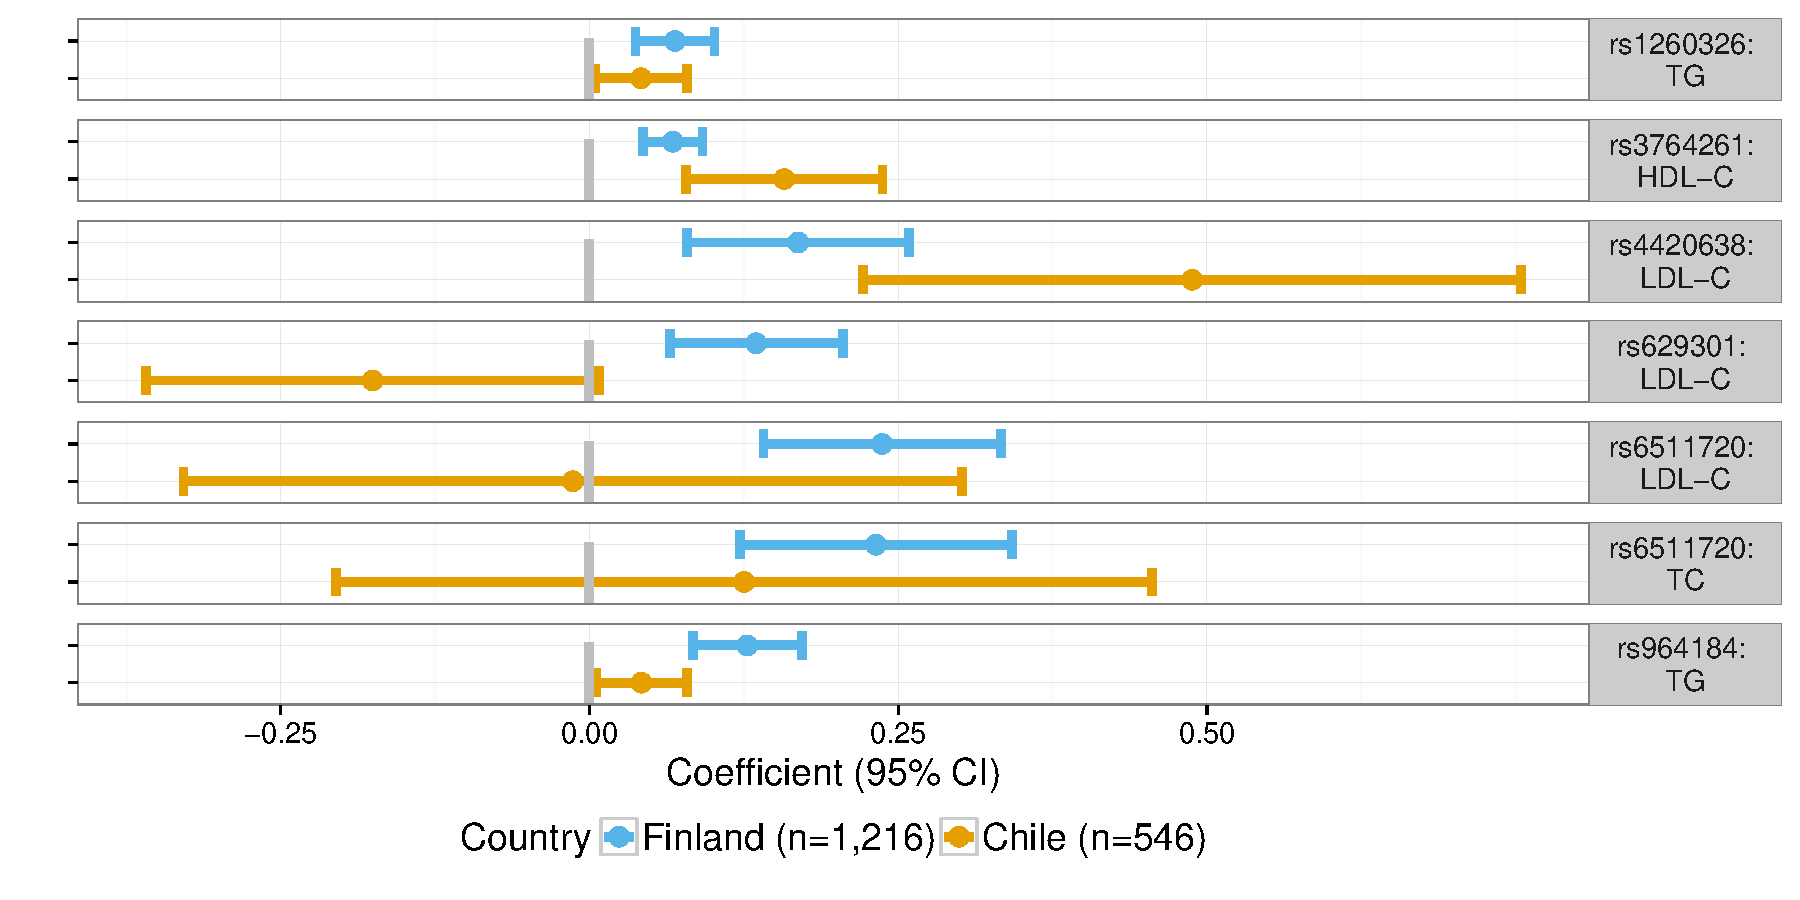
\includegraphics[width=\maxwidth]{figure/fig-assoc-2-1} 

          \small Figure 1. Candidate single variant tests of association by variant and sample

\end{frame}
% 
% \subsection{Figure 1}
% \begin{frame}{Results, Figure 1}
% 
%             \begin{itemize}
%             \item \raggedright  Majority of single variants tested in Chilean sample have concordant direction of associations.
%               \begin{itemize}
%                 \item Two LDL-C variants in opposite direction.
%                 \end{itemize}
%               \end{itemize}
% 
% \end{frame}


% ------------------------------


\subsection{Figure 2}  
\begin{frame}{wGRS has stronger association for each lipid outcome in Chilean versus Finnish sample except LDL-C.}
        
        % Second figure
        % %%%%%%%%%%%%%%%%%%%%%%%%%%%%%%%%%%%%%%%%%%%%%%%%%%
\vskip-1em
\centering

% Run code chunk from tables-slides.R to make table from summary statistics run on Kure



\begin{knitrout}
\definecolor{shadecolor}{rgb}{0.969, 0.969, 0.969}\color{fgcolor}
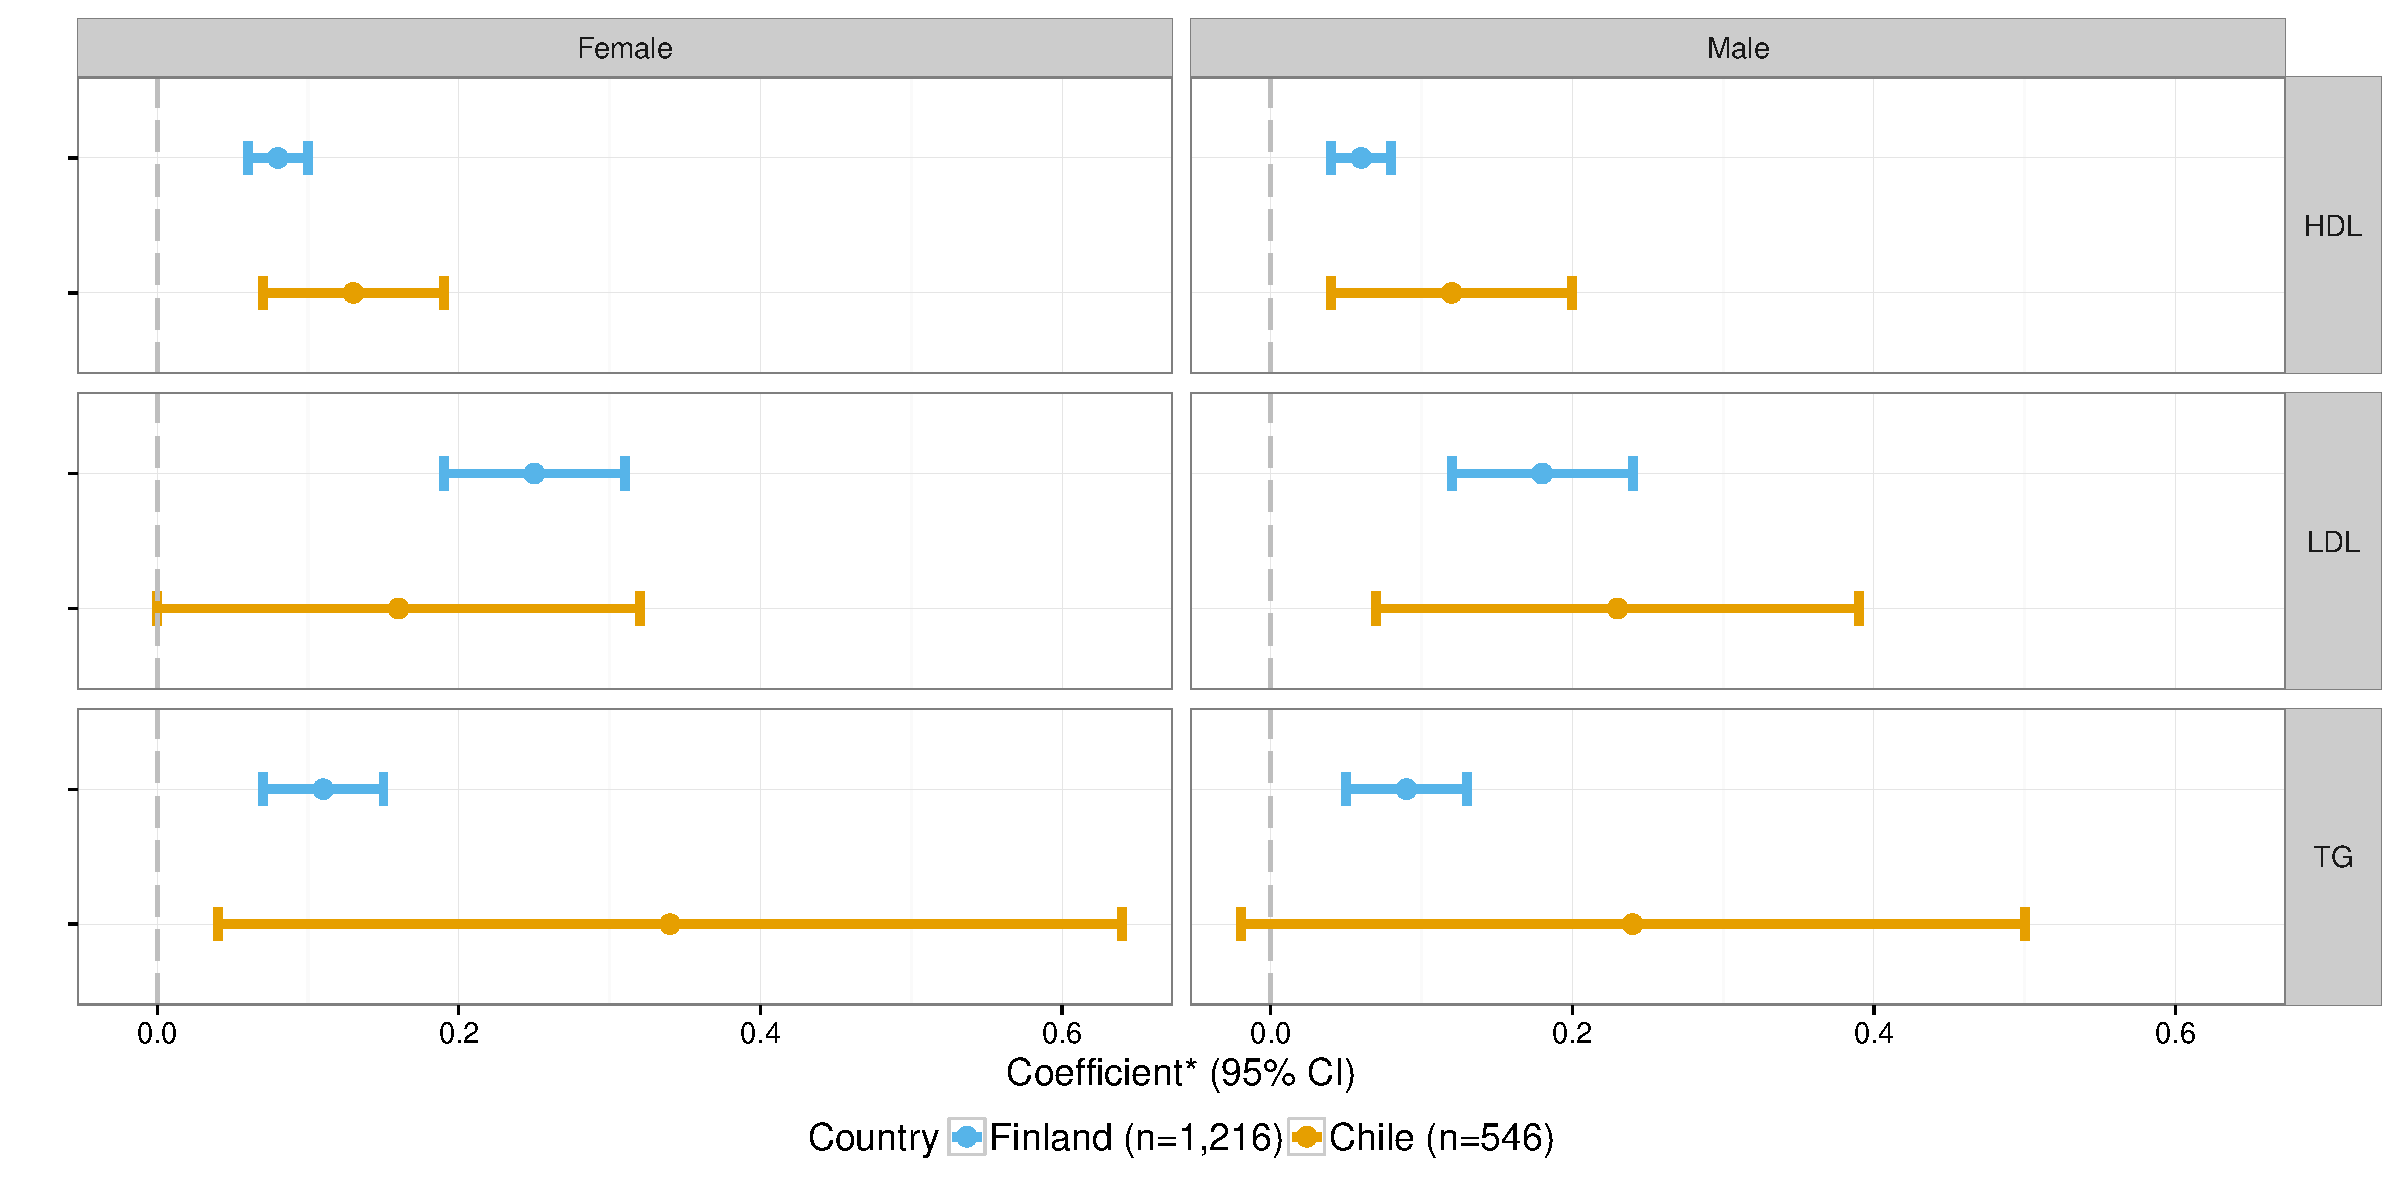
\includegraphics[width=\maxwidth]{figure/fig3-2-1} 

\end{knitrout}

        
        \begin{addmargin}[0.1cm]{0cm}
        \begin{flushleft}
        \footnotesize{*Coefficients represent change in outcome per 1 SD change in wGRS, adjusted for first five principal components representing ancestry.}
        \end{flushleft}
        \end{addmargin}
    \small Figure 2. wGRS regression coefficients by sample and sex

\end{frame}

% \begin{frame}{Results, Figure 2}
%         \begin{itemize}
%             \item \raggedright  wGRS has stronger association for each lipid outcome in Chilean versus Finnish sample except LDL-C for females.
%             \end{itemize}
% 
% \end{frame}

% ------------------------------

\begin{frame}{ LDL-C-related variants explain much less variance in Chilean sample.}
        % Third figure
        % %%%%%%%%%%%%%%%%%%%%%%%%%%%%%%%%%%%%%%%%%%%%%%%%%%

% Run code chunk from tables-slides.R to make table from summary statistics run on Kure


        
\vskip-0.5em
        \centering

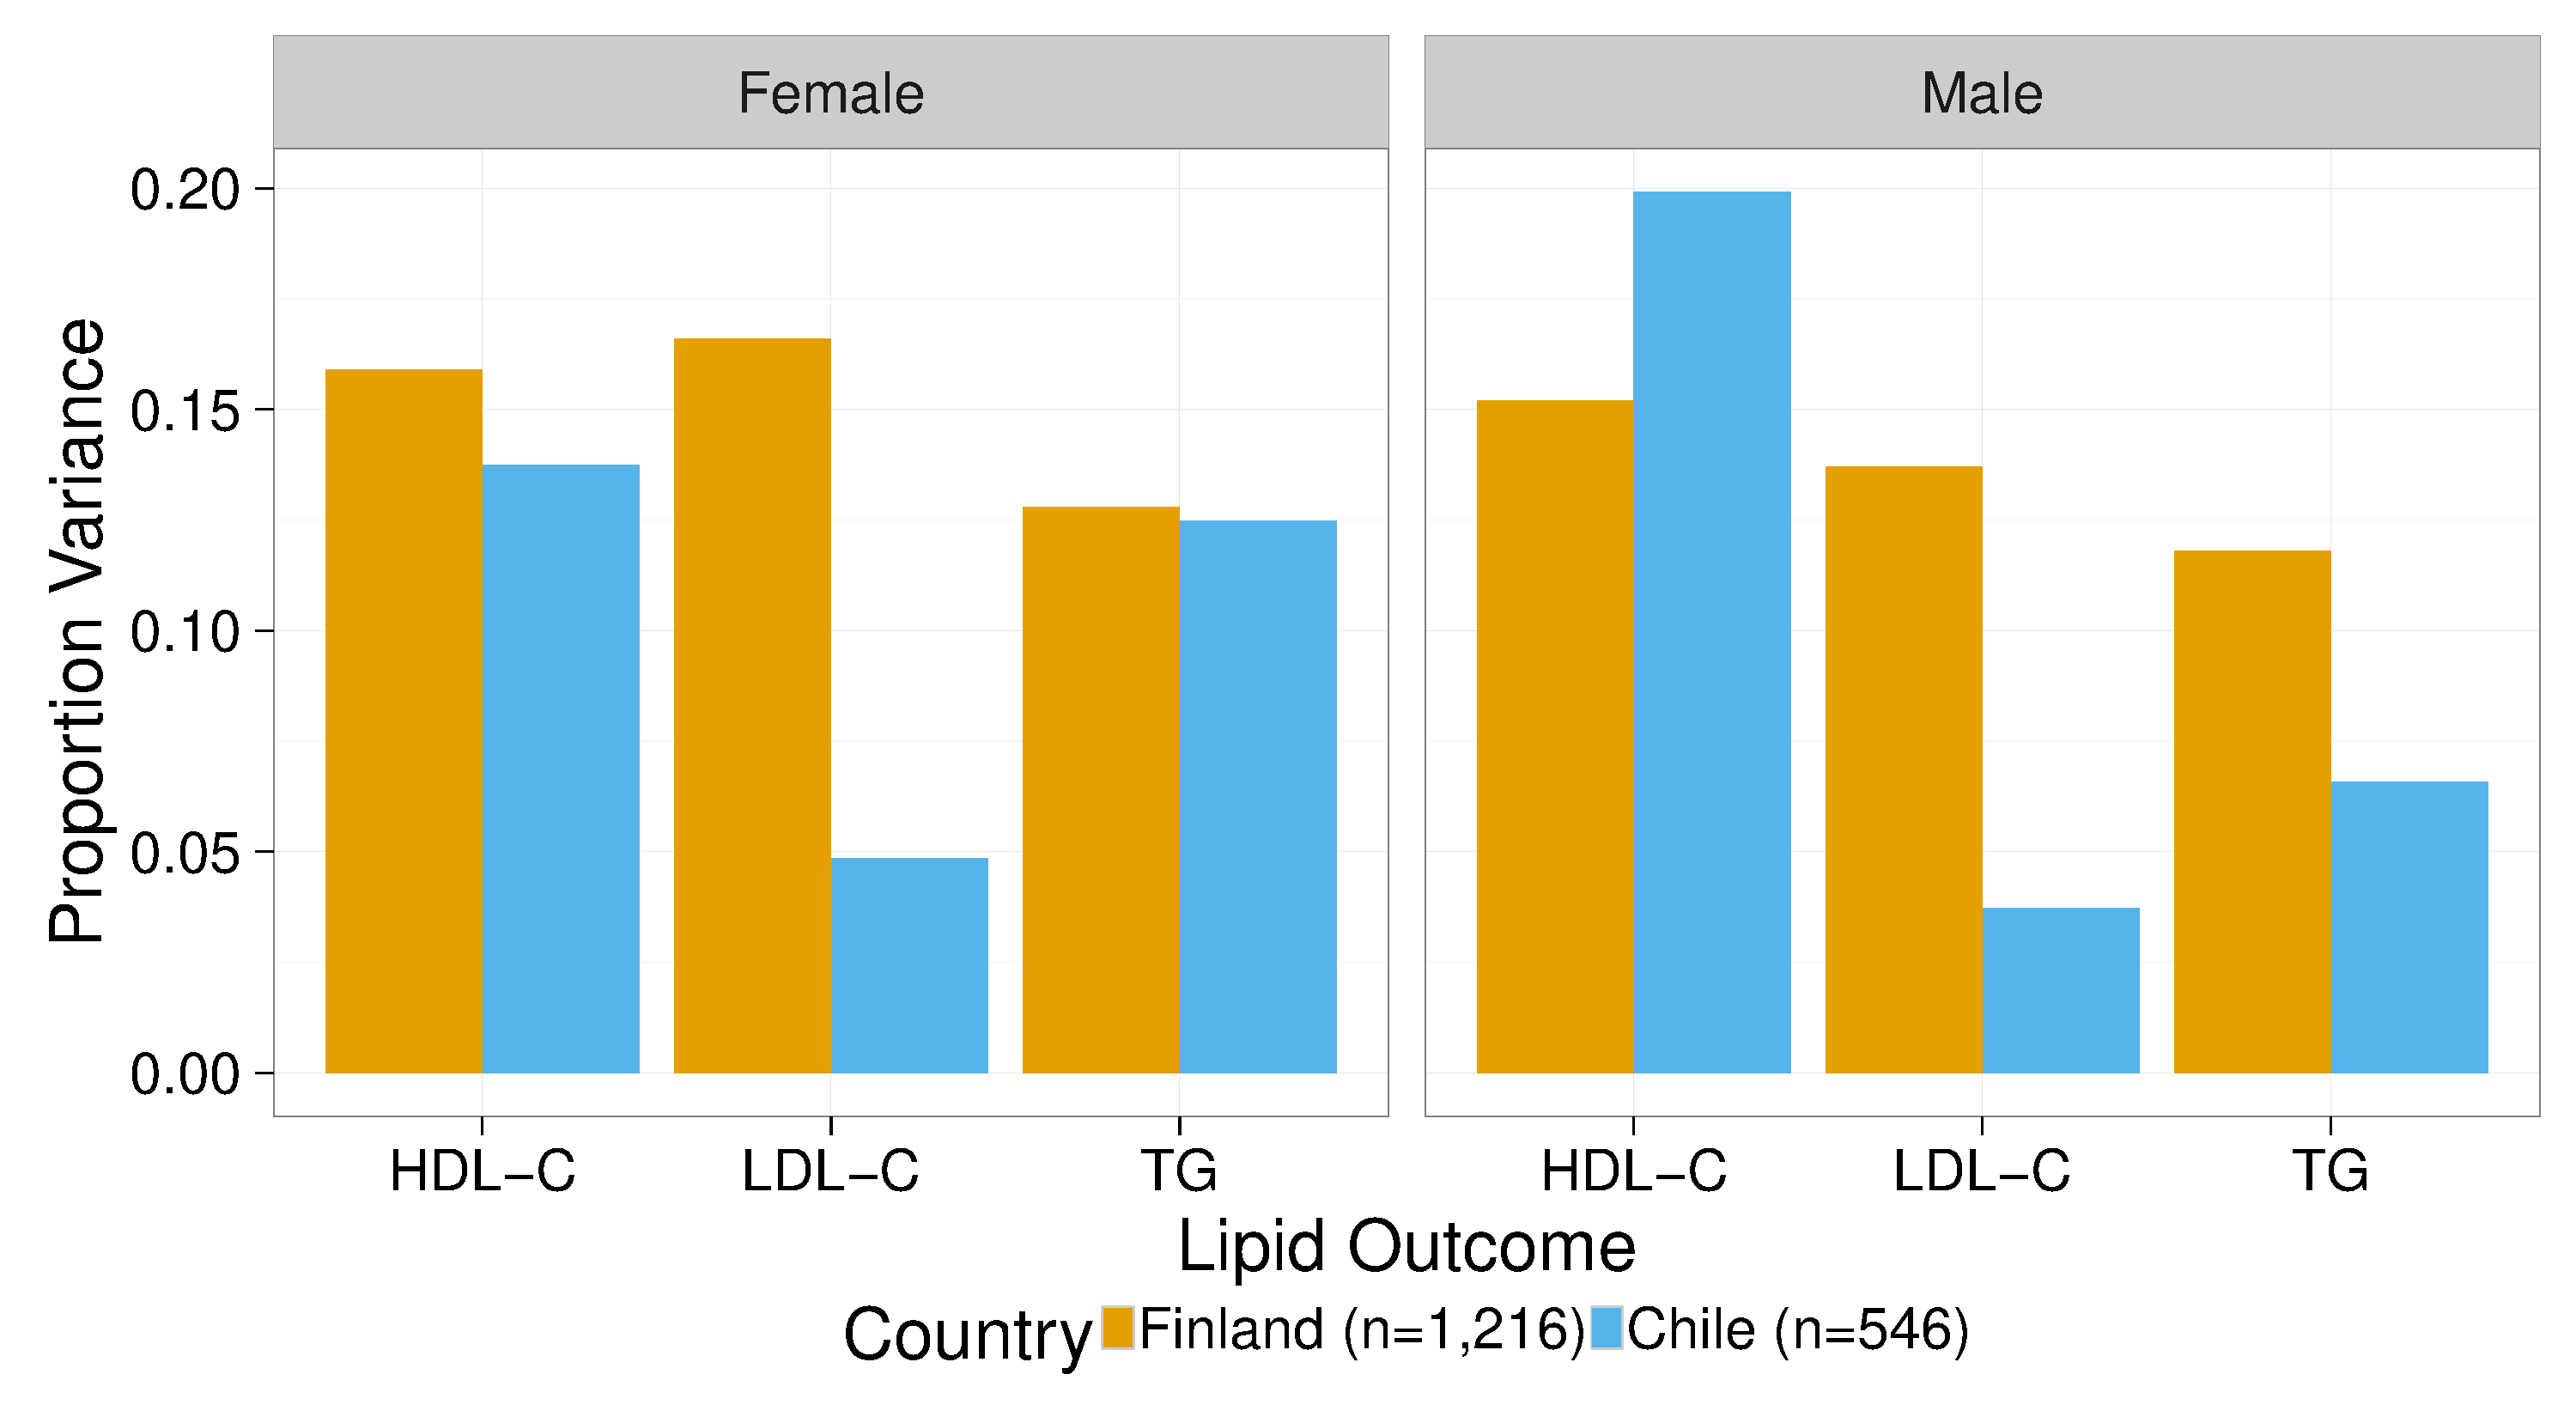
\includegraphics[width=\maxwidth]{figure/fig2-2poster-1} 

\small Figure 3. Proportion of lipid traits variance explained by lipid-related variants, by sex

\end{frame}

% \begin{frame}{Results, Figure 3}
% %        \begin{mdframed}[style=MyFrame]
%           \begin{itemize}
%             \item \raggedright LDL-C-related variants explain much less variance in Chilean sample.
%             \end{itemize}
% %            \end{mdframed}
%         
% \end{frame}

% ------------------------------
\section{Summary}
\subsection{Summary}

\begin{frame}{Summary}
        
          \begin{itemize}
            \item We found meaningful and statistically significant associations relating lipid loci in a HL cohort of Chilean adolescents despite the potential for bias given different haplotype structures across populations.

              \item Significant associations support concordance of effects across European and HL populations found in adults for these loci\footfullcite{weissglas-volkov_genomic_2013}.
                \item  LDL-C associations are not statistically significant although selections based on power under assumptions of European effect size.
                \begin{itemize} 
                  \item Possibility that either linkage disequilibrium or different causal variant is responsible for the failure to detect a difference\footfullcite{below_genome-wide_2016}.
                \end{itemize}

    \item Genetic risk evident in childhood presents across different populations, emphasizing younger ages as a point for intervention.
            \end{itemize}
  \end{frame}



\end{document}
